\subsubsection{Página de projeto}

É na página de projeto que um aluno pode consultar todas as informações sobre um projeto de uma unidade curricular da qual faz parte.

Sendo um projeto uma das principais entidades do sistema, esta é uma página com que tivemos especial cuidado, para permitir que o utilizador encontre a informação e ações que procura, se uma forma simples e eficiente.\\

Num plano principal, optou-se por colocar as informações do projeto, com a descrição do projeto e as restrições dos elementos para os grupos de trabalho.

Logo após as informações de projeto, são listadas todas as fases do projeto, numa  linha temporal, explicitando as fases concluídas, a fase atual e as fases seguintes.

Como a avaliação de uma fase é uma das informações mais relevantes para o utilizador, optou-se por colocar, já nesta listagem, essa informação.

É importante referir que, ao clicar numa fase, o utilizador acede a uma página com informações detalhadas sobre essa fase, é também nessa página que o utilizador pode efetuar entregas.

No painel da direita, ao lado das informações do projeto, podem ser encontrados um conjunto de atalhos para páginas de muito interesse para o utilizador, o enunciado do projeto, a gestão de grupos de trabalho, a gestão de fases e entregas e as avaliações.

Ainda no mesmo painel, podem ser encontradas notificações relativas ao projeto, o grupo de trabalho atual e uma lista de últimas entregas.\\

Na Figura~\ref{fig:student_project} pode ser consultada uma imagem demonstrativa da página desenvolvida.

\begin{figure}[H]
  \centering
  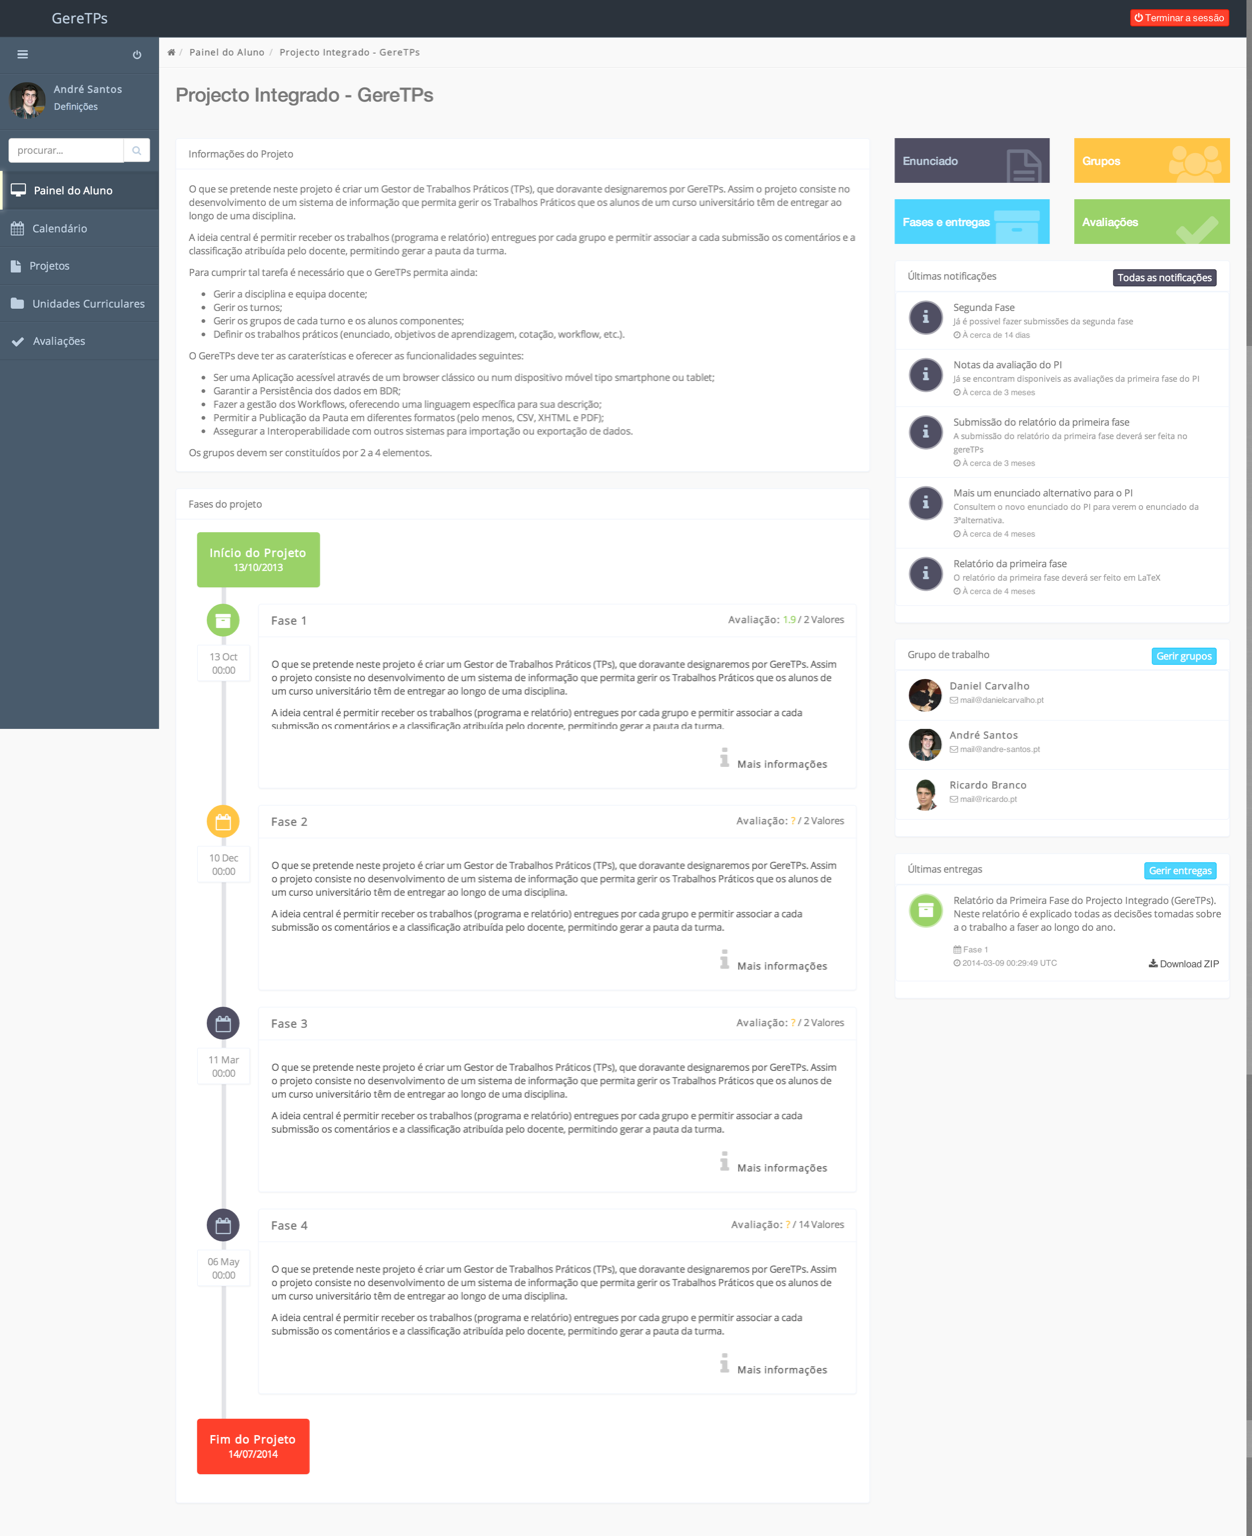
\includegraphics[width=.8\textwidth,center]{images/implementacao/alunos/project}
  \caption{Página de projeto}
  \label{fig:student_project}
\end{figure}
